\chapter{Experiment 2: Valid execution traces}\label{sec:ch5}

In the experiment from \autoref{sec:ch4}, we designed a tool to test generated
systems, \textit{i.e.} testing invalid execution trace. However, testing valid
execution trace can also provide valuable results to test whether the generated
system conforms to the specification. In this chapter, we discuss how we are
testing the valid execution traces and how to solve the limitations of the
experiment from \autoref{sec:ch4}.

\section{More complex specifications}\label{sec:ch5-complex-spec}
In the previous approaches is only the account specification used. In this
experiment, we are going to use more complex specifications, complex in the
sense that they depend and interact with each other.

We are going to use the
same account specification from \autoref{fig:account-spec}. As an addition to
account specification, we use a transaction specification. Via this
specification money can be transferred between two accounts.
The \textit{Rebel} implementation of the transaction specification \footnote{\url{https://github.com/cwi-swat/rebel/blob/e58590c7f51f59e7ee6443bb89ef09dff6febab6/rebel-core/examples/simple_transaction/Transaction.ebl}} is shown in \autoref{fig:transaction-spec}.
As shown in the transaction specification, it contains more fields than the
account specification. The two remarkable fields are from and to, both are of
the \textit{IBAN} type. The type \textit{IBAN} is a built-in \textit{Rebel}
type.~\cite[p.~3]{stoel_storm_vinju_bosman_2016} Note that after the type
definition an annotation is given to specify a reference to another
specification, in this case, account specification. The fields to and from are
being used to indicate between whom the transaction takes place.

According to the transaction specification, the transaction first
needs to be started. When a transaction is in the state validated, and a booking
cannot be made, the transition \textit{fail} can be used to put the transaction in its
final state failed. To successfully complete a transaction is the transition
\textit{book} used. In comparison to the account specification, does the transaction
specification two final states, which are booked and failed. When the final
state booked or failed is reached, then there is no further action allowed.
Note that the transaction specification does not have an invariant.

Another difference in the transaction specification is that event definitions
can contain sync expressions. From the previous event definitions, we have only
seen pre- and postconditions. Sync expressions are used for synchronisation.
These sync expressions are also translated to \gls{smt} formulas.

The sync expressions translated to the \gls{smt} solver are also logical formulas.
These formulas do not have logic about synchronisation. Of course, the \gls{sut} has
implemented synchronisation for these transitions. So it is possible to also
test synchronisation in the \gls{sut}. There are also several studies which report
that \gls{smt}-based approaches to model checking can be used to test distributed
algorithms.~\cite{konnov2015you, alberti2015smt, mccaffrey2016verification}

% Sync expressions are used to synchronously execute a blocking transition without the interference of other related transitions which may change the state of the instances used within the sync expressions. \unsure{which is better? or a paper ref?}

The \textit{book} transition uses the synchronisation feature to express sync
operations (see \autoref{fig:transaction-book-event}). A sync operation is here
used to withdraw an amount from one account and to deposit to another account.

% \info{new scala generator, two-phase commit for distribution.}
% \info{explain sync stuff and about distribution, look at implementation of
% sync in smt. Theoretically it is possible to find errors in distributed stuff.}

\begin{sourcecode}[h!]
\begin{lstlisting}[]
specification Transaction {
	fields {
		id: Integer @key
		amount: Money
		from: IBAN @ref=Account
		to: IBAN @ref=Account
	}

	events {
		start[]
		book[]
		fail[]
	}

	lifeCycle {
		initial uninit -> validated: start
		validated    -> booked: book
					-> failed: fail
		final booked
		final failed
	}
}
\end{lstlisting}
\caption{Transaction specification}\label{fig:transaction-spec}
\end{sourcecode}
\FloatBarrier

\begin{sourcecode}[h!]
\begin{lstlisting}[]
event book() {
	sync {
		Account[this.from].withdraw(this.amount);
		Account[this.to].deposit(this.amount);
	}
}
\end{lstlisting}
\caption{\textit{book} event definition from transaction specification}\label{fig:transaction-book-event}
\end{sourcecode}
\FloatBarrier

\section{Method}
% The simulation of Rebel is able to translate a single step to SMT formulas.

As discussed in \autoref{sec:research-method}, a model testing approach is
already done to test existing banking systems. Although, in this approach, it
was only possible to test the \gls{sut} interactively using the simulation. In this
approach are the traces from the \gls{smt} solver used to check whether the
\gls{sut} accepts the execution from the trace and whether it behaves as the
specification.~\cite[p.~5]{stoel_storm_vinju_bosman_2016}

By using the traces, it also solves the problems from the previous experiment.
With the use of traces, we know exactly which possible transitions the
\gls{smt} solver has performed. Then these transitions can be performed in the \gls{sut}.
So, in this approach, we are going to use the traces to check the behaviour of the
\gls{sut}.

\subsection{Evaluation criteria}\label{sec:ch5-eval-criteria}

\subsubsection{Bugs}
In this approach we are using the traces from the \gls{smt} solver to test the
\gls{sut}, thus testing what should be possible according to the specification.
The expectation here is to find bugs in the \gls{sut} which does not accept the
execution from the traces. For instance, the generated pre- or postconditions
are not satisfied by the transition from the traces or the generated
postcondition which leads to different results. An example of this is the bug
that we have found in \autoref{sec:bug-close-account}.

In \autoref{sec:ch5-complex-spec} we discussed that we are going to use more
complex specification which implements synchronisation. As discussed, it is
possible to test synchronisation in the \gls{sut}. Thus the expectation is to
find faults in the implementation of the synchronisation in the \gls{sut}.

In \autoref{sec:ch2-codegen} we discussed the Codegen-Akka generator. The
\gls{sut} from the generator uses Akka as Actor Model. Akka is a toolkit
which is used for building concurrent, distributed and resilient
message-driven systems.~\cite[p.~4]{roestenburg2016akka}

It is difficult to build and test distributed systems, according to the
study~\cite[p.~1]{mccaffrey2016verification}, this has two main reasons: partial
failure and asynchrony. When components fail along the way that results into
incomplete results or data is called partial failure. Within a system,
asynchrony is the non-determinism of ordering and timing. That is to say; the
expectation is to find faults in partial failure and asynchrony. Not only is the
expectation to find these faults in the Codegen-Akka, but also in the other code
generators since these code generators implements also synchronisation. For
instance, the Codegen-Javadatomic uses \gls{cqrs} where the commands are
executed asynchronously.

At the time of experimenting, a new version of the Codegen-Akka is
released. The new version implements \gls{2pc}, which is a synchronisation
protocol~\cite[p.~3204]{al2009two}. A protocol like \gls{2pc} is also referred
to as an \gls{acp}. The essence of \gls{acp} is to achieve global atomicity. The
protocol ensures a unanimous final outcome of a distributed transaction,
regardless of the failures that may occur.~\cite[p.~3204]{al2009two} In our
case, the expectation is to find bugs in synchronisation where the \gls{sut}
does not produce a unanimous final outcome. However, the traces from the
\gls{smt} solver must also be unanimous to the \gls{sut}.

\subsubsection{Efficiency}
In the experiment from \autoref{sec:ch5}, we have seen that with the use of
checking, the result from the \gls{smt} solver varies. For the testing
framework, it's unknown whether the performed transition is the same as the
computed transition by the \gls{smt} solver. The \gls{smt} solver is
smarter/better in checking the satisfiability of a given constraints. This,
limitation from the previous experiment can be solved by using the traces from
the \gls{smt} solver.

By using the traces for testing, the same path computed by the \gls{smt} solver
are performed in the \gls{sut} and we can check whether the given
execution is possible in the \gls{sut}. Thus the expectation is to perform the
same transition from the traces should be performed in the \gls{sut}.
However, it may take longer to test all transitions from specifications as each
transition needs to be tested and some transitions require an initial state for
which transitions need to be performed to reach this state.

\subsubsection{Coverage}
In this experiment, the simulation is used to test transitions. Since
the simulation can test single steps, it is expected to test all
transitions of a specification.

As discussed, this experiment is going to use more complex specifications,
\textit{e.g.}, specifications which depend and interact with each other. With
the use of the simulation, it is expected to test transitions which depend and
interact with other specifications.

With the criteria bugs, we discussed that it is expected to find faults in
partial failure and asynchrony. These characteristics may lead to not testing
transitions. To illustrate what is meant, let us look at the case of partial
failure within the \textit{book} transition. When components fail along the way
during the transitions to reach the initial state for the \textit{book}
transition, it may result in incomplete results or data. This leads to the
inability to test the \textit{book} transition.

\section{Approach}

The process of the testing approach with the simulation is shown in
\autoref{fig:simulation-testing}. This process starts first with the creation of
a specification. This experiment uses the account and transaction specifications
which are already defined.

Once the specification is defined, the specifications
are being built, \textit{i.e.}, \gls{csts} are produced of
these specifications. Using these \gls{csts}, the code generator generates the code,
which is then the \gls{sut}.

When the \gls{sut} is generated from the \gls{csts}, the \gls{sut} can be tested by the test
framework. The test case generator traverses the \gls{csts} of the specifications to
generates test cases for all transitions. Using the information from the \gls{csts},
the simulation is requested for a test case for a chosen transition. The
simulation provides then a trace (test case) for the requested transition.

To test the \gls{sut} using the generated test cases, the data
from these test cases are provided to the test case adapter. Finally, the test
case adapter communicates this data to the \gls{sut}.

\begin{figure}[h!]
  \centering
  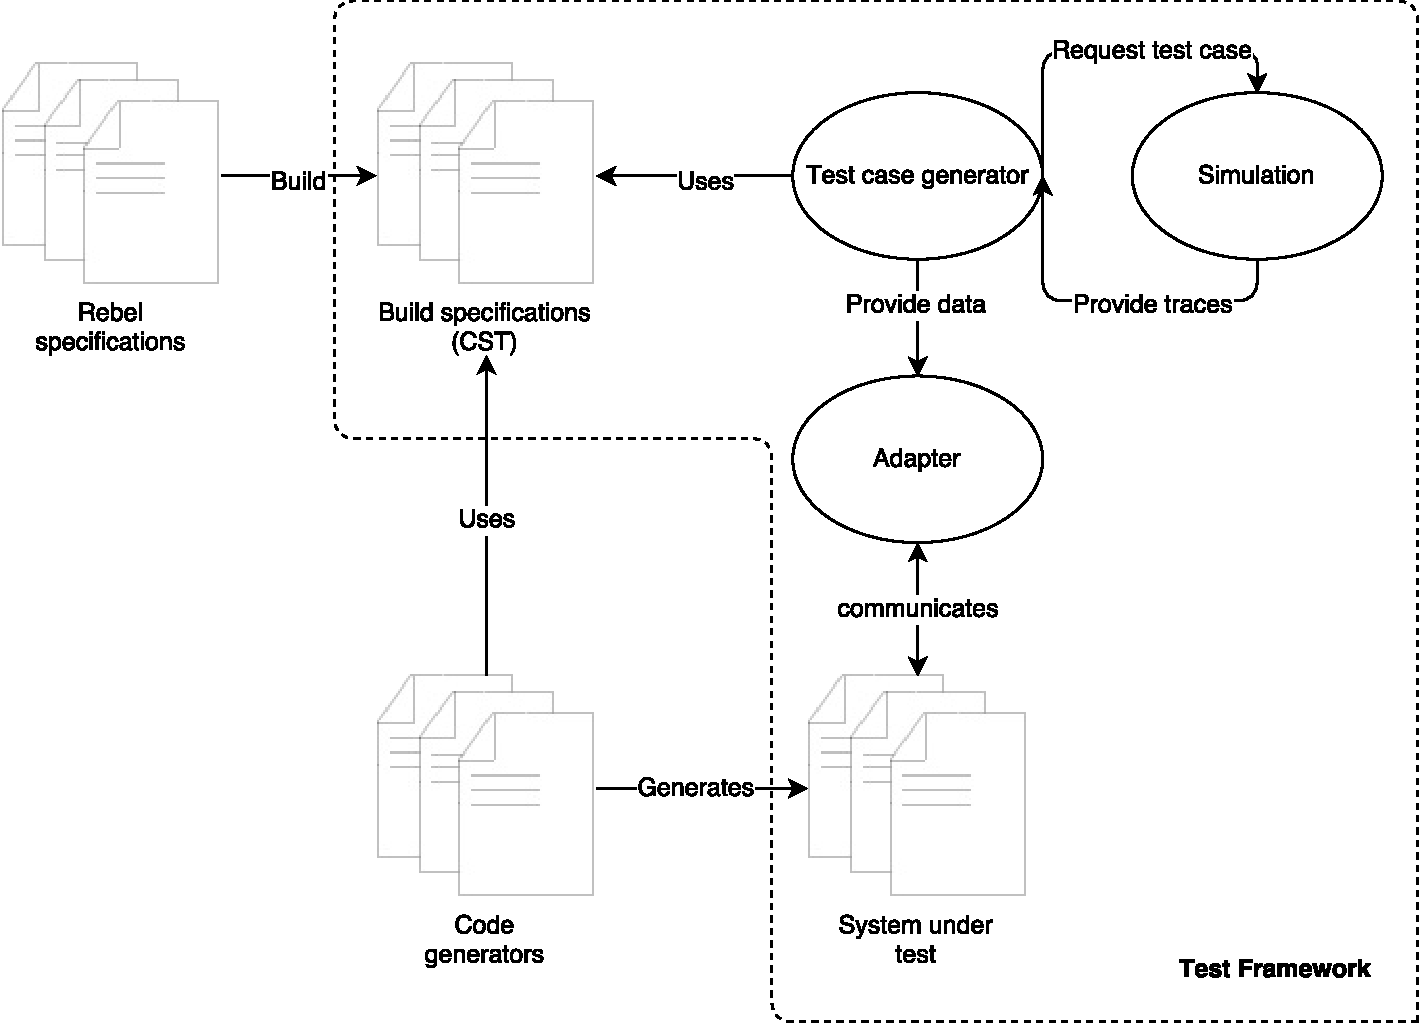
\includegraphics[width=\linewidth{}]{figures/simulation-diagram.pdf}
  \caption{Testing approach with simulation}\label{fig:simulation-testing}
\end{figure}
\FloatBarrier

To playback the steps from a given trace on the \gls{sut}, we are going to split every
transition into three steps as in the
study~\cite[p.~6]{stoel_storm_vinju_bosman_2016}:
\begin{enumerate}
\item \textbf{pre-transition check} Check whether the current state from the \gls{sut}
is conform to the current state from the trace
\item \textbf{transition check} Execute the given transition from the trace on
the \gls{sut}
\item \textbf{post-transition check} Check whether the new state from the \gls{sut} is
conform to the new state from the trace
\end{enumerate}

The transition function for the simulation looks as follows: $p(s_{1}, s_{2})$,
which has the pre- and postcondition of the to be executed transition
\cite[p.~6]{stoel_storm_vinju_bosman_2016}. The current state $s_{1}$ holds the
constraints of the current values of the simulated specification. Hereafter, to
execute the transition, the user is asked to provide the data for the transition
parameters.

Before using the simulation, two challenges need to be solved: defining the
current state for a given transition and providing the transition parameters
data values. These challenges are discussed in the paragraphs below.

\subsection{Pre-transition check}

\subsubsection*{Current state}\label{sec:ch5-current-state}

The pre-transition checks entail the check for the current state of the \gls{sut} is
conform to the current state from the trace. Although with the simulation it is
only possible to reason about individual steps. For some transitions a current
state is required, \textit{e.g.}, an account needs to be blocked first to
unblock it. To make use of the simulation, the current state needs to be defined
to check whether the step can be made from the current state. This is also the
case in the \gls{sut} since a current state needs to be initialised first before the
transition is performed.

To initialise the current state in the \gls{sut} checking can be used. By defining
the current state with checking, the current state is checked, and a valid trace
is given by the model checker when the current state is satisfiable. So for
every transition, a tebl needs to be generated for the state to reach
(current state) to perform the transition. Although there are some caveats with
the use tebl.

When a state to reach is defined for checking, the identifiers for the entities
are unique within that trace. For example for
\autoref{fig:tebl-opened-simple-account}, the identifier for the opened account
from the traces is \textit{NL10INGB0000001}. The identifiers for similar
entities are auto-incremented, \textit{e.g.}, when an additional account entity
is specified in \autoref{fig:tebl-opened-simple-account} the identifier is then
\textit{NL10INGB0000002}. This is not only the case with IBAN numbers but also
with Integer, String, etc. This is not a problem when a single transition is
tested. When multiple transitions are tested and even when there are multiple
entities, this will result in collisions of existing entities with the same
identifiers. Note also that the generated IBAN numbers by the \gls{smt} solver are
also not valid.

The invalid IBAN numbers is not a problem for the
checking since checking is only used to reason about possible traces. However,
this does not hold in the \gls{sut} since \gls{sut} is a banking system and here it must
conform to the IBAN standards. It is possible with checking to define the
properties of an entity, \textit{e.g.}, the IBAN for an account.

To solve the
problem with the collision of existing entities, a random identifier should be
given for each entity. Therefore, for each type like Integer, is a random
generator implemented. This generator generates a random identifier which is
used as the identifier for the entities in checking. Unlike the basic types,
IBAN is a more complex type to generate since the type should conform to the
IBAN standards. Therefore, Iban4j~\cite{iban4j} is used to generate random IBAN
account numbers which are compliant to the ISO\_13616 and ISO\_9362 standards.

Another pitfall with the use of checking is the use of more complex
specifications, \textit{e.g.}, the transaction specification. With such
specifications, it is possible to have a reference to another specification. In
the case of the transaction specification involves two references, namely
account specification. To use checking in such specifications must be taken into
account the references to other specifications. Which means that for every
referencing specification in checking, imports need to be resolved and defined,
and the entity needs to be defined with an identifier. Note that these
identifiers should be again random. Otherwise, it will cause collisions of
existing entities.

Altogether, a generated tebl for checking the current state looks as follows in
\autoref{fig:tebl-gen-validated-transaction}. Note that the configurable
time-out is set to four since the states from the account and transaction
specification are reachable within four steps. The determination of the
configurable time-out per specification is left as future work.

When the current state is defined, the generated tebl is given to the model
checker. When the current state is satisfiable are the traces used to perform
the transitions in the \gls{sut}. This is in more depth described in the section
\autoref{sec:ch5-traces}. Performing each step from a trace entails the three
steps to test and perform the transition.

\begin{sourcecode}[h!]
\begin{lstlisting}[]
module simple_transaction.Test

import simple_transaction.Transaction
import simple_transaction.Account

state doCheck {
  validated Transaction with id == 65227;

  Account with accountNumber == NO3631174980518;
  Account with accountNumber == LB404150J311SB1FJV5KL1MKYAY4;
}

check doCheck reachable in max 4 steps;
\end{lstlisting}
\caption{Generated tebl for the transition book}\label{fig:tebl-gen-validated-transaction}
\end{sourcecode}
\FloatBarrier

\subsubsection*{Current state values}
After the current state is defined, the same approach from the previous chapter
can be used to check whether it is satisfiable. The \gls{smt} solver returns whether the
current state is satisfiable with the traces, including the instances with its
values.

To provide transition parameters data to the simulation is the last step taken
with its instances. The last step is taken because the last step is the
transition which led to the current state, which is going to be used by the
simulation. The values from these instances of the simulated specifications are
given to the current state $s_{1}$.

The simulation checks only whether the step can be made from the given current
state, it does not check whether the current state is reachable. With the use of
checking for the current state is the current state checked whether this is
satisfiable.

\subsection{Transition check}
% Execute the given transition from the trace on the SUT

\subsubsection*{Transition parameters data values}
Since simulation is used for reasoning about individual steps, that explains why
the transition parameters data values for the chosen transition should be
provided by the user. As discussed earlier is in the model testing approach
of the study \cite[p.~6]{stoel_storm_vinju_bosman_2016} chosen for interactively
using the simulation.

Manually providing the transition parameters data values
is not relevant for us, since we intend to test automatically the \gls{sut}.
Certainly, these values can be generated randomly, but it should satisfy the
pre- and postconditions for the chosen transition. However, it would be
better to let the \gls{smt} solver fill these values, taking into account the pre- and
postconditions of the chosen transition. At the time of the publication of the
study~\cite{stoel_storm_vinju_bosman_2016}, this was not possible in the simulation, so
the simulation should be slightly modified.

In cooperation with the author of the study~\cite{stoel_storm_vinju_bosman_2016} is this feature added to the simulation.~\footnote{\url{https://github.com/cwi-swat/rebel/commit/0d29eb30a82cc5dd6d8be750daa4a24e4e2786be}}
The simulation is now able that both state variables and transition variables
can be left open, in the sense of using the expression \textit{ANY}. When the
expression \textit{ANY} is used, the \gls{smt} solver will fill a value for the
corresponding transition parameter, satisfying the pre- and postconditions for
the chosen transition. \unsure{what about expression as iban?}

\subsubsection*{Traces}\label{sec:ch5-traces}
A valid trace is a chain of valid transitions from one state to the next state
\cite[p.~5]{stoel_storm_vinju_bosman_2016}. The trace may contain multiple steps,
\textit{e.g.}, to unblock an account, an account needs first to be opened and
blocked. This requires after executing each step; the step needs to be tested,
in the sense of automatically repeating the testing process. Each step from the
traces has instances with its state and values.

The instances are specific
for that step, the results after performing the step are given in the state and
values for instance. A trace for simulation contains the state before
performing the transition, the step (transition), and then the state after
performing the step.

After everything is defined for the simulation, the simulation can test whether
it can make the single step. The simulation then works as follows
\cite[p.~6]{stoel_storm_vinju_bosman_2016}:
\begin{enumerate}
\item Check whether it is possible to satisfy the constraints of the chosen
transition given the current state and the transition parameters data values of
the event: $p(s_{1}, s_{2})$
\item Check whether the invariants hold in the state after the transition:
$P(s2)$.
\end{enumerate}

When this step can be made, with the use of traces, the step can be played on
the \gls{sut}. Therefore, \textit{JSON} should be generated for the chosen
transition. This is the responsibility of the test case adapter, which is
explained more in depth in \autoref{sec:ch5-adapter}. To generate the
\textit{JSON}, the transition parameters data values and
the transition name are read from the trace step. At last, the endpoint is
determined for the given step, and the generated JSON is sent to the endpoint.

\subsection{Post-transition check}
% Check whether the new state from the SUT is conform to the new state from the trace

Since a trace contains the instances before and after the step, this can be used
in the post-transition check to test the \gls{sut}. As a result, we can check after or
before performing the step, whether the \gls{sut} behaves similarly as the
simulated/checked specification.

To check whether the new state from the \gls{sut} is
conform to the trace, the state and values from the instances are read after
performing the transition. The endpoint is then determined to retrieve the state
of these instances in the \gls{sut}. Then, the results of these instances from the \gls{sut}
and trace are compared to find any misbehaviour in the \gls{sut}.
\improvement{check all instances}

\subsubsection{Normalisation}

Before a \textit{Rebel} specification is checked or simulated is the specification
normalised. This normalisation process is done to make the \gls{smt} formulas easier
and also to give it partially semantics
\cite[p.~5]{stoel_storm_vinju_bosman_2016}. Desugaring the life cycle is part of
the normalisation process. The life cycle is desugared to strengthen the pre-
and postconditions of the transitions with the life cycle information.
Therefore, are two fields added, \textit{\_state} and \textit{\_step}, to the fields of the
specification. To each state and event is a distinct identity assigned. The
identity of the current state is assigned to the \textit{\_state} field, and the identity
of the transition which led to the current state is assigned to the field
\textit{\_step}. This results into that the original life cycle can be expressed, by
adding constraints on the \textit{\_state} and \textit{\_step} fields to the transitions pre- and
postconditions \cite[p.~5]{stoel_storm_vinju_bosman_2016}.

The newly added fields
are also present within the trace from the \gls{smt} solver. In our case, we only use
the \textit{\_state} field, because we already know which transition led to the current
state. To compare the current state from the \textit{\_state} field, it needs to be
sugared back to compare it to the \gls{sut}.
% Adding Frame Conditions. To guard the fields that are not changed by the event frame conditions are added (Jack- son 2012). These frame conditions make sure that a field has the same value after the transition as before.

\subsubsection{Test case adapter}\label{sec:ch5-adapter}
As discussed in the code generation section, the request made to the \gls{api} of the
\gls{sut} are "standardized", but the response from the \gls{sut} is not. For the
post-transition check, it is necessary to check the new state in the \gls{sut}.
Therefore, an adapter needs to be defined to communicate the results of the
traces with the \gls{sut}.

An adaptor is often used in model-based testing
approaches.~\cite{utting2012taxonomy, tretmans2003torx}
The adapter is a component that concretises the test inputs and abstraction of
test outputs, \textit{i.e.}, the adapter adapts the abstract test data to the
concrete \gls{sut} interface.~\cite[p.~4]{utting2012taxonomy}
On request of the test case generator, the adaptor provides inputs to, and
receives outputs from the \gls{sut}. The adapter encodes and decodes the
abstract actions from the test case adapter to concrete actions for the
\gls{sut}.~\cite[p.~5]{tretmans2003torx} This leads to that the adapter is
dependent on the specification and the \gls{sut}.

According to the study~\cite[p.~4]{utting2012taxonomy}, an adaptor is a concept,
and that does not mean that an adapter needs to be a separate software component.
The adapter may be integrated within the test scripts. The test script is code
which executes a test case, abstracts the response from the \gls{sut} and
creates the verdict. In our case, the test case adapter is integrated into the
test script, which is the test case generator.

The decision is made to only implement a test case adapter for the code generator
Codegen-Akka since this is a more mature code generator and frequently used for
experiments within ING Bank.

\section{Results}\label{sec:ch5-results}

\subsection{Codegen-Akka}\label{sec:ch5-run-codegenakka}

The results of the test run are shown in
\autoref{fig:ch5-res-codegenakka-account} and
\autoref{fig:ch5-res-codegenakka-transaction}. From this result, we can conclude
that the test for the \textit{close} transition has failed.

\begin{table}[h!]
\centering
\begin{tabular}{ccc}
\toprule
\textbf{Transition to test} & \textbf{Current state} & \textbf{Transition} \\ \midrule
openAccount                 & \cmark{}               & \cmark{}            \\
withdraw                    & \cmark{}               & \cmark{}            \\
deposit                     & \cmark{}               & \cmark{}            \\
interest                    & \cmark{}               & \cmark{}            \\
block                       & \cmark{}               & \cmark{}            \\
unblock                     & \cmark{}               & \cmark{}            \\
close                       & \cmark{}               & \xmark{}            \\ \bottomrule
\end{tabular}
\caption{Results: testing account specification transitions}\label{fig:ch5-res-codegenakka-account}
\end{table}
\FloatBarrier

\begin{table}[h!]
\centering
\begin{tabular}{ccc}
\toprule
\textbf{Transition to test} & \textbf{Current state} & \textbf{Transition} \\ \midrule
start                       & \cmark{}               & \cmark{}            \\
book                        & \cmark{}               & \cmark{}            \\
fail                        & \cmark{}               & \cmark{}            \\ \bottomrule
\end{tabular}
\caption{Results: testing transaction specification transitions}\label{fig:ch5-res-codegenakka-transaction}
\end{table}
\FloatBarrier

\subsection{Codegen-Javadatomic}
The results of the test run are shown in
\autoref{fig:ch5-res-codegendatomic-account} and
\autoref{fig:ch5-res-codegendatomic-transaction}. From this result, we can
conclude again that the test for the \textit{close} transition has failed. Remarkable is
that also the \textit{interest} transition has failed.

\begin{table}[h!]
\centering
\begin{tabular}{ccc}
\toprule
\textbf{Transition to test} & \textbf{Current state} & \textbf{Transition} \\ \midrule
openAccount                 & \cmark{}               & \cmark{}            \\
withdraw                    & \cmark{}               & \cmark{}            \\
deposit                     & \cmark{}               & \cmark{}            \\
interest                    & \cmark{}               & \xmark{}            \\
block                       & \cmark{}               & \cmark{}            \\
unblock                     & \cmark{}               & \cmark{}            \\
close                       & \cmark{}               & \xmark{}            \\ \bottomrule
\end{tabular}
\caption{Results: testing account specification transitions}\label{fig:ch5-res-codegendatomic-account}
\end{table}
\FloatBarrier

\begin{table}[h!]
\centering
\begin{tabular}{ccc}
\toprule
\textbf{Transition to test} & \textbf{Current state} & \textbf{Transition} \\ \midrule
start                       & \cmark{}               & \cmark{}            \\
book                        & \cmark{}               & \cmark{}            \\
fail                        & \cmark{}               & \cmark{}            \\ \bottomrule
\end{tabular}
\caption{Results: testing transaction specification transitions}\label{fig:ch5-res-codegendatomic-transaction}
\end{table}
\FloatBarrier

\subsection{Codegen-Scala-ES}
The results of the test run are shown in
\autoref{fig:ch5-res-codegendatomic-account} and
\autoref{fig:ch5-res-codegendatomic-transaction}. Again the test for the
transition \textit{close} has failed, but also for the transition interest.

\begin{table}[h!]
\centering
\begin{tabular}{ccc}
\toprule
\textbf{Transition to test} & \textbf{Current state} & \textbf{Transition} \\ \midrule
openAccount                 & \cmark{}               & \cmark{}            \\
withdraw                    & \cmark{}               & \cmark{}            \\
deposit                     & \cmark{}               & \cmark{}            \\
interest                    & \cmark{}               & \xmark{}            \\
block                       & \cmark{}               & \cmark{}            \\
unblock                     & \cmark{}               & \cmark{}            \\
close                       & \cmark{}               & \xmark{}            \\ \bottomrule
\end{tabular}
\caption{Results: testing account specification transitions}\label{fig:ch5-res-codegenscalaes-account}
\end{table}
\FloatBarrier

\begin{table}[h!]
\centering
\begin{tabular}{ccc}
\toprule
\textbf{Transition to test} & \textbf{Current state} & \textbf{Transition} \\ \midrule
start                       & \cmark{}               & \cmark{}            \\
book                        & \cmark{}               & \cmark{}            \\
fail                        & \cmark{}               & \cmark{}            \\ \bottomrule
\end{tabular}
\caption{Results: testing transaction specification transitions}\label{fig:ch5-res-codegenscalaes-transaction}
\end{table}
\FloatBarrier

\subsection{Distributed Codegen-Akka}\label{sec:ch5-run-dist-codegenakka}
In \autoref{sec:ch5-run-codegenakka} we have seen the test results of the
Codegen-Akka generator. In this test run is the \gls{sut} run as single nodes,
both the Scala system and Cassandra.

With this test run, we will run the \gls{sut} distributed generated by the
Codegen-Akka generator. The results of the test run are shown in
\autoref{fig:ch5-res-dist-codegenscalaes-account} and
\autoref{fig:ch5-res-dist-codegenscalaes-transaction}. It is noteworthy that all
tests fail.

\begin{table}[h!]
\centering
\begin{tabular}{ccc}
\toprule
\textbf{Transition to test} & \textbf{Current state} & \textbf{Transition} \\ \midrule
openAccount                 & \xmark{}               & \xmark{}            \\
withdraw                    & \xmark{}               & \xmark{}            \\
deposit                     & \xmark{}               & \xmark{}            \\
interest                    & \xmark{}               & \xmark{}            \\
block                       & \xmark{}               & \xmark{}            \\
unblock                     & \xmark{}               & \xmark{}            \\
close                       & \xmark{}               & \xmark{}            \\ \bottomrule
\end{tabular}
\caption{Results: testing account specification transitions}\label{fig:ch5-res-dist-codegenscalaes-account}
\end{table}
\FloatBarrier

\begin{table}[h!]
\centering
\begin{tabular}{ccc}
\toprule
\textbf{Transition to test} & \textbf{Current state} & \textbf{Transition} \\ \midrule
start                       & \xmark{}               & \xmark{}            \\
book                        & \xmark{}               & \xmark{}            \\
fail                        & \xmark{}               & \xmark{}            \\ \bottomrule
\end{tabular}
\caption{Results: testing transaction specification transitions}\label{fig:ch5-res-dist-codegenscalaes-transaction}
\end{table}
\FloatBarrier

\section{Analyse}

\subsection{Codegen-Akka}
The experiment uses in this test run the Codegen-Akka generator.
Investigating the test run, it seems to be that all transitions are tested
successfully, except the transition \textit{close}. Also, there seems to be a
limitation in testing the state of a specification.

\subsubsection{\textit{close} transition}\label{sec:close-no-test-codegenakka}

The result of \textit{close} transition test is shown in
\autoref{fig:result-codegenakka-close}. As shown on line number 28 is
constructing the current state for the \textit{close} transition successful. Then the
simulation is asked to simulate the \textit{close} transition, but according to the
traces of the simulation, the simulation was not able to make the step. The
simulation returns only the state before the transition.

\begin{sourcecode}[h!]
\begin{lstlisting}[]
Test transition close
opened -> close -> closed

0:
  now = 14 Aug 2017, 13:49

  instance: simple_transaction.Account, key = FO9402337176862639
    ?
    ?
    var accountNumber (type: IBAN) (uninitialized)
    var balance (type: Money) (uninitialized)

1:
  now = 14 Aug 2017, 13:49
  step: simple_transaction.Account.openAccount
    var initialDeposit (type: Money) = EUR50.00
    Transition to state = opened
    Identified by accountNumber = FO9402337176862639

  instance: simple_transaction.Account, key = FO9402337176862639
    State = opened
    ?
    var accountNumber (type: IBAN) = FO9402337176862639
    var balance (type: Money) = EUR50.00

Endpoint: /Account/FO9402337176862639/OpenAccount
JSON payload: { "OpenAccount": { "initialDeposit":"EUR 50.00" } }
Response: ("body":"CommandSuccess(OpenAccount(50.00 EUR))","isSuccessful":"true","message":"OK",
"errorBody":"","code":"200")

1:
  now = 12 Jul 2016, 12:00:00

  instance: simple_transaction.Account, key = FO9402337176862639
    State = opened
    ?
    var accountNumber (type: IBAN) = FO9402337176862639
    var balance (type: Money) = EUR50.00
\end{lstlisting}
\caption{No test generated for \textit{close} transition}\label{fig:result-codegenakka-close}
\end{sourcecode}
\FloatBarrier

As discussed earlier, the precondition of the \textit{close} transition is that there
should be no remaining balance as shown in \autoref{fig:account-close-event}.
On line number 15 of the test run is shown that the simulation makes the step to
open an account with a balance of 50 euros. Afterwards are no transitions
performed. Thus this current state does not satisfy the precondition of the
\textit{close} transition. That is the reason why the simulation was not able to perform the
transition since the given values from the current state to $s_{1}$ were not
satisfying for $s_{2}$.

The generated tebl for the current state is shown in
\autoref{fig:tebl-gen-validated-transaction}. Only the state to reach is
specified with the identifier of the account. As we have seen the event definition
of \textit{openAccount} in \autoref{fig:account-openaccount-event}, the account
must be opened with a balance of 50 euros.

To conclude, the simulation was not able to test the transition \textit{close} since the
precondition of this transition is not satisfied in the postcondition of $s_{1}$.
This also holds for testing \gls{sut}s by other code generators. In other
words, this limitation is the result of the test approach

\begin{sourcecode}[h!]
\begin{lstlisting}[]
module simple_transaction.Test

import simple_transaction.Account

state doCheck {
  opened Account with accountNumber == AD3517248539N3OTXZIDF13H;
}

check doCheck reachable in max 4 steps;
\end{lstlisting}
\caption{Generated tebl for the transition book}\label{fig:tebl-gen-validated-transaction}
\end{sourcecode}
\FloatBarrier

\subsubsection{State testing}

In \autoref{fig:result-not-found-state} is the test run shown of the transition
\textit{book}. Only the first transition is shown in this figure. As you can
see on line 42 is the \textit{openAccount} transition performed. On the line
below is shown that the request is successful. On line 44 is an error message
shown which tells that it is not able to find the state of the opened account.
Note the question mark in this message. This error message is part of the
post-transition check where the new state of the \gls{sut} is tested. On line number
35 is the instance account shown after the transition and on the line below you
can see the same question mark. Both question mark relates to each other, which
is the state of a given specification.

In testing single specifications, \textit{e.g.}, in
\autoref{fig:result-codegenakka-close}, we have seen that the state is present
from the result of the \gls{smt} solver. In this case, the model checker/simulation
does not return the state when multiple instances are involved. This also
happens in the \textit{start} and \textit{fail} transitions.

\begin{sourcecode}[h!]
\begin{lstlisting}[]
Test transition book
validated -> book -> booked

0:
  now = 15 Aug 2017, 11:17
  instance: simple_transaction.Transaction, key = 97691
    ?
    ?
    var id (type: Integer) (uninitialized)
    var from (type: IBAN) (uninitialized)
    var amount (type: Money) (uninitialized)
    var to (type: IBAN) (uninitialized)

  instance: simple_transaction.Account, key = CY4945493642LWV6W6RZ3EDZSGTB
    ?
    ?
    var accountNumber (type: IBAN) (uninitialized)
    var balance (type: Money) (uninitialized)

  instance: simple_transaction.Account, key = NL60IZNV8233056080
    ?
    ?
    var accountNumber (type: IBAN) (uninitialized)
    var balance (type: Money) (uninitialized)

1:
  now = 15 Aug 2017, 11:17
  step: simple_transaction.Account.openAccount
    var initialDeposit (type: Money) = EUR50.00
    Transition to state = opened
    Identified by accountNumber = NL60IZNV8233056080

  // ... other instances from the state above

  instance: simple_transaction.Account, key = NL60IZNV8233056080
    ?
    ?
    var accountNumber (type: IBAN) = NL60IZNV8233056080
    var balance (type: Money) = EUR50.00

Endpoint: /Account/NL60IZNV8233056080/OpenAccount
JSON payload: { "OpenAccount": { "initialDeposit":"EUR 50.00" } }
Response: ("body":"CommandSuccess(OpenAccount(50.00 EUR))","isSuccessful":"true","message":"OK",
  "errorBody":"","code":"200")
Could not find state ?, expected  "state":{"?":{}}
\end{lstlisting}
\caption{State not found for entities}\label{fig:result-not-found-state}
\end{sourcecode}
\FloatBarrier

% https://github.com/ING-CoreBank-University/ing-codegen-datomic/commit/4ebcd4df0a90fc10451562a6a43c3fcd8891fce3
\subsection{Codegen-Javadatomic}\label{sec:bug-interest-javadatomic}

In this test run is the Javadatomic generator used. After investigating the test
run, it seems to be that testing the transition \textit{interest} fails. As you can see
in \autoref{fig:result-javadatomic-interest} on line number 55, the request made
for \textit{interest} transition is not successful, and the HTTP status code returned 400
is returned. Constructing the current state for the \textit{interest} transition seems to
be successful (see line number 28). According to the simulation, on line number
40, the step interest is made with a negative percentage (- 7709). On line
number 47, you can see the instance after performing the interest step, which
resulted into an account entity with the state opened and with a negative
balance. To conclude, the transition \textit{interest} is possible according to the
simulation.

Although, the request made for the transition \textit{interest} is not
successful, and when we take a look at the account in the \gls{sut}, the account looks
as follows in \autoref{fig:interest-opened-account-json}. The state of the
account is still opened, and the balance seems to be the same when the account
was opened. From looking at the state of the account, the \textit{interest} transition
is not performed in the \gls{sut} and the state of the account is the same as before
performing the transition.

% less than percentage

\begin{sourcecode}[h!]
\begin{lstlisting}[]
Test transition interest
opened -> interest -> opened

0:
  now = 13 Jul 2017, 12:26

  instance: simple_transaction.Account, key = MD14FLBLJOYGVJMDUZVKLU4C
    ?
    ?
    var accountNumber (type: IBAN) (uninitialized)
    var balance (type: Money) (uninitialized)

1:
  now = 13 Jul 2017, 12:26
  step: simple_transaction.Account.openAccount
    var initialDeposit (type: Money) = EUR50.00
    Transition to state = opened
    Identified by accountNumber = MD14FLBLJOYGVJMDUZVKLU4C

  instance: simple_transaction.Account, key = MD14FLBLJOYGVJMDUZVKLU4C
    State = opened
    ?
    var accountNumber (type: IBAN) = MD14FLBLJOYGVJMDUZVKLU4C
    var balance (type: Money) = EUR50.00

Endpoint: /Account/MD14FLBLJOYGVJMDUZVKLU4C/OpenAccount
JSON payload: { "OpenAccount": { "initialDeposit":"EUR 50.00" } }
Response: ("body":"{\"iban\":\"MD14FLBLJOYGVJMDUZVKLU4C\"}","isSuccessful":"true",
  "message":"OK","errorBody":"","code":"200")

1:
  now = 12 Jul 2016, 12:00:00

  instance: simple_transaction.Account, key = MD14FLBLJOYGVJMDUZVKLU4C
    State = opened
    ?
    var accountNumber (type: IBAN) = MD14FLBLJOYGVJMDUZVKLU4C
    var balance (type: Money) = EUR50.00

2:
  now = 12 Jul 2016, 12:00:00
  step: simple_transaction.Account.interest
    var currentInterest (type: Percentage) = (- 7709)
    Transition to state = opened
    Identified by accountNumber = MD14FLBLJOYGVJMDUZVKLU4C

  instance: simple_transaction.Account, key = MD14FLBLJOYGVJMDUZVKLU4C
    State = opened
    ?
    var accountNumber (type: IBAN) = MD14FLBLJOYGVJMDUZVKLU4C
    var balance (type: Money) = - EUR3804.50

Endpoint: /Account/MD14FLBLJOYGVJMDUZVKLU4C/Interest
JSON payload: { "Interest": { "currentInterest":"-77.09" } }
Response: ("body":"","isSuccessful":"false","message":"Bad Request","errorBody":"","code":"400")
\end{lstlisting}
\caption{Failing test on \textit{interest} transition with the use of javadatomic generator}\label{fig:result-javadatomic-interest}
\end{sourcecode}
\FloatBarrier

\begin{sourcecode}[h!]
\begin{lstlisting}[]
{
	"_id": 17592186045441,
	"_version": 1,
	"_status": "OPENED",
	"accountNumber": {
		"iban": "MD14FLBLJOYGVJMDUZVKLU4C"
	},
	"balance": {
		"value": 50.00,
		"currency": "EUR"
	}
}
\end{lstlisting}
\caption{Account state in the \gls{sut} after performing the \textit{interest} transition}\label{fig:interest-opened-account-json}\end{sourcecode}
\FloatBarrier

The event definition for the \textit{interest} transition is given in
\autoref{fig:account-interest-event}. This event definition states that the
precondition is that the \textit{currentInterest} must be less than or equal
10\%, and the postcondition is that the balance must be changed after applying
the interest. The generated transition parameter \textit{currentInterest},
- 7709, satisfies also this precondition.

\begin{sourcecode}[h!]
\begin{lstlisting}[]
function singleInterest(balance: Money, interest: Percentage): Money =  balance * interest;

event interest[maxInterest: Percentage = 10%](currentInterest: Percentage) {
  preconditions {
    currentInterest <= maxInterest;
  }
  postconditions {
    new this.balance == this.balance + singleInterest(this.balance, currentInterest);
  }
}
\end{lstlisting}
\caption{\textit{Interest} event definition from account specification}\label{fig:account-interest-event}
\end{sourcecode}
\FloatBarrier

Now we know that we have discovered a bug since the simulated transition is
conform to the specification, we want to know where this misbehaviour occurs and
which code is not correctly generated. The generated code for the \textit{interest} event
definition from \autoref{fig:account-interest-event} contains the following
check in \autoref{fig:java-gen-interest-pre}. The generated code for the
preconditions seems to be good since it uses a \textit{isLessOrEqualThan}
function with the given interest percentage. Looking at the log file created by
the \gls{sut}, the exception \textit{BuildCASTransactionException} is thrown when
performing the \textit{interest} transition, which is the exception from
\autoref{fig:java-gen-interest-pre}. So the generated code seems to be good, but
the function used for validating the interest returns an inappropriate value,
which throws the exception.

\begin{sourcecode}[h!]
\begin{lstlisting}[language=Java]
if(! (isLessOrEqualThan(currentInterest, 10 /* % */))) {
  throw new BuildCASTransactionException("Predicate did not hold: InterestTransaction: currentInterest
	  <= 10%");
}
\end{lstlisting}
\caption{Code in Java}\label{fig:java-gen-interest-pre}
\end{sourcecode}
\FloatBarrier

The function \textit{isLessOrEqualThan} is shown in
\autoref{fig:java-less-or-equal-check}. This function takes two parameters, both
of the type \textit{BigDecimal}, and compares the \textit{lhs} to the
\textit{rhs}; this result should be greater or equal than zero. This function
is not correctly defined since this is the definition of the function
\textit{isGreaterOrEqualThan}. This code is not generated but is part of the
fixed code.

Clearly, we have discovered a bug in the \gls{sut} for the transition
interest. As discussed in \autoref{sec:ch3-evalution}, it is possible to have
bugs in the fixed code. With this experiment and testing the Javadatomic
generator, we can conclude that we have found a bug in the fixed code.

\begin{sourcecode}[h!]
\begin{lstlisting}[language=Java]
public static boolean isLessOrEqualThan(BigDecimal lhs, BigDecimal rhs) {
  return lhs.compareTo(rhs) >= 0;
}
\end{lstlisting}
\caption{Code in Java}\label{fig:java-less-or-equal-check}
\end{sourcecode}
\FloatBarrier

\subsection{Codegen-Scala-ES}\label{sec:bug-interest-scalaes}
% Interest squants dimensionlessdata

This test run tests the \gls{sut} generated by the Scala-ES generator. Looking at the
test run, as the test runs for the Javadatomic generator, it seems to be
that the transition \textit{interest} fails. The results of the test run are shown in
\autoref{fig:result-scalaes-interest}. Line number 51 shows the failing request
for the \textit{interest} transition; an error message is returned with the HTTP status
code 400. Also, in this test run is construction the current state for the
\textit{interest} transition successful (see line number 26). In this test run, the
simulation has generated the same trace for the \textit{interest} transition as for the
Javadatomic generator. The state of the account in the \gls{sut} looks as follows in
\autoref{fig:interest-opened-account-scalaes-json}. Also here the state of the
account opened, and the balance seems to be the same when the account was opened.
So, the performed \textit{interest} transition has failed, and the state of the account
is the same before performing the transition.

\begin{sourcecode}[h!]
\begin{lstlisting}[]
Test transition interest
opened -> interest -> opened

0:
  now = 12 Aug 2017, 18:29
  instance: simple_transaction.Account, key = MT58PDLQ09015VOS06LIF4Q525NRO1I
    ?
    ?
    var accountNumber (type: IBAN) (uninitialized)
    var balance (type: Money) (uninitialized)
1:
  now = 12 Aug 2017, 18:29
  step: simple_transaction.Account.openAccount
    var initialDeposit (type: Money) = EUR50.00
    Transition to state = opened
    Identified by accountNumber = MT58PDLQ09015VOS06LIF4Q525NRO1I

  instance: simple_transaction.Account, key = MT58PDLQ09015VOS06LIF4Q525NRO1I
    State = opened
    ?
    var accountNumber (type: IBAN) = MT58PDLQ09015VOS06LIF4Q525NRO1I
    var balance (type: Money) = EUR50.00

Endpoint: /Account/MT58PDLQ09015VOS06LIF4Q525NRO1I/OpenAccount
JSON payload: { "OpenAccount": { "initialDeposit":"EUR 50.00" } }
Response: ("body":"{\"iban\":\"MT58PDLQ09015VOS06LIF4Q525NRO1I\"}","isSuccessful":"true",
"message":"OK","errorBody":"","code":"200")

1:
  now = 12 Jul 2016, 12:00:00
  instance: simple_transaction.Account, key = MT58PDLQ09015VOS06LIF4Q525NRO1I
    State = opened
    ?
    var accountNumber (type: IBAN) = MT58PDLQ09015VOS06LIF4Q525NRO1I
    var balance (type: Money) = EUR50.00
2:
  now = 12 Jul 2016, 12:00:00
  step: simple_transaction.Account.interest
    var currentInterest (type: Percentage) = (- 7709)
    Transition to state = opened
    Identified by accountNumber = MT58PDLQ09015VOS06LIF4Q525NRO1I

  instance: simple_transaction.Account, key = MT58PDLQ09015VOS06LIF4Q525NRO1I
    State = opened
    ?
    var accountNumber (type: IBAN) = MT58PDLQ09015VOS06LIF4Q525NRO1I
    var balance (type: Money) = - EUR3804.50

Endpoint: /Account/MT58PDLQ09015VOS06LIF4Q525NRO1I/Interest
JSON payload: { "Interest": { "currentInterest":"-77.09" } }
Response: ("body":"","isSuccessful":"false","message":"Bad Request",
"errorBody":"com.fasterxml.jackson.databind.JsonMappingException: Can not construct instance of
squants.Dimensionless: no String-argument constructor&#x2F;factory method to deserialize from String
value (&#x27;-77.09&#x27;)\n at [Source: io.undertow.servlet.spec.ServletInputStreamImpl@578015db;
line: 1, column: 35] (through reference chain: nl.ing.corebank.dto.
account.Interest[&quot;currentInterest&quot;])","code":"400")
\end{lstlisting}
\caption{Failing test on \textit{interest} transition with the use of Scala-ES generator}\label{fig:result-scalaes-interest}
\end{sourcecode}
\FloatBarrier

\begin{sourcecode}[h!]
\begin{lstlisting}[]
{
   "_id":"nl.ing.corebank.aggregates.AccountAggregate$|077708cd-769a-48ec-8006-d607241c4f45",
   "_version":1,
   "_state":"OpenedState",
   "accountNumber":{
      "iban":"MT58PDLQ09015VOS06LIF4Q525NRO1I"
   },
   "balance":"50.00 EUR"
}
\end{lstlisting}
\caption{Account state in the \gls{sut} after performing the \textit{interest} transition}\label{fig:interest-opened-account-scalaes-json}
\end{sourcecode}
\FloatBarrier

Likewise, the Javadatomic generator, we have discovered a bug in the \gls{sut}, since
the simulated transition is not conform to the specification. To know where this
bug occurs and which code is not properly generated, the response from the
\textit{interest} transition request gives an error message. According to the error
message, the \gls{sut} is not able to construct the instance of \textit{Dimensionless}
for the transition parameter \textit{currentInterest}. This error seems to occur
in the class \textit{Interest}, which is shown in
\autoref{fig:scala-gen-interest-json}. The parameter \textit{currentInterest}
indeed uses the type \textit{Dimensionless} here.

\begin{sourcecode}[h!]
\begin{lstlisting}[language=scala]
@JsonRootName(value = "Interest")
@JsonCreator
case class Interest(@JsonProperty("currentInterest") currentInterest: Dimensionless)
\end{lstlisting}
\caption{Code in Scala}\label{fig:scala-gen-interest-json}
\end{sourcecode}
\FloatBarrier

The class from \autoref{fig:scala-gen-interest-json} is used in
\autoref{fig:scala-gen-interest-request}. The \textit{interest} method handles
the \textit{interest} transition and as you can see is the class \textit{Interest} used
as the second parameter. This class is used to bind the interest parameter as a
type of the \textit{Interest} class.

In short, we have discovered a bug in the \gls{sut}
for the \textit{interest} transition. The \textit{interest} transition bug in the Javadatomic
generator belongs to the fixed code category, but in this case, for the Scala-ES
generator, the bug belongs to the injected code category, since the
\textit{Interest} class is generated and injected in the generated code.

\begin{sourcecode}[h!]
\begin{lstlisting}[language=scala]
@POST
@Consumes(Array[String](MediaType.APPLICATION_JSON))
@Produces(Array[String](MediaType.APPLICATION_JSON))
@Path("/{accountNumber}/Interest")
def interest(@Suspended asyncResponse: AsyncResponse,
  @PathParam("accountNumber") accountNumber: IBAN, interest: Interest): Unit = {
\end{lstlisting}
\caption{Code in Scala}\label{fig:scala-gen-interest-request}
\end{sourcecode}
\FloatBarrier

% \subsection{Two-phase commit}
% datetime transaction

\subsection{Distributed Codegen-Akka}\label{sec:bug-dist-nodes}
In this test run is again the Codegen-Akka generator used, but the \gls{sut}
runs distributed. By running the \gls{sut} as multiple nodes, two Scala system
nodes and one Cassandra node, we can focus more on testing the unanimous final
outcome of the \gls{sut}s. Therefore, the pre-transition check and transition
check are performed in the first node (Node 1). The post-transition check is
performed in the second node (Node 2). In previous experiments, the three steps
are performed to execute and test transitions in a single node. By performing
the post-transition check on Node 2, it can be checked whether the
\gls{sut} produces a unanimous final outcome.

To investigate the failing tests, we discuss the test result for the transition
\textit{interest}. The results of the test run are shown in
\autoref{fig:result-dist-codegenakka-interest}. The test for the current state
as well as the transition fails for the transition \textit{interest}.
As shown on line number 27 the request for constructing the current state is
successful. As part of the post-transition check, checking whether the new state
from the \gls{sut} is conform to the new state from the trace fails
(see line number 29-30). This also applies to the \textit{interest} transition;
the transition succeeds but the post-transition check fails.

\begin{sourcecode}[h!]
\begin{lstlisting}[]
Test transition interest
opened -> interest -> opened

0:
  now = 18 Sep 2017, 08:57

  instance: simple_transaction.Account, key = FO1227539908389742
    ?
    ?
    var accountNumber (type: IBAN) (uninitialized)
    var balance (type: Money) (uninitialized)
1:
  now = 18 Sep 2017, 08:57
  step: simple_transaction.Account.openAccount
    var initialDeposit (type: Money) = EUR50.00
    Transition to state = opened
    Identified by accountNumber = FO1227539908389742

  instance: simple_transaction.Account, key = FO1227539908389742
    State = opened
    ?
    var accountNumber (type: IBAN) = FO1227539908389742
    var balance (type: Money) = EUR50.00

Endpoint: /Account/FO1227539908389742/OpenAccount
JSON payload: { "OpenAccount": { "initialDeposit":"EUR 50.00" } }
Response: ("body":"CommandSuccess(OpenAccount(50.00 EUR))","isSuccessful":"true","message":"OK",
  "errorBody":"","code":"200")
Could not find state opened, expected  "state":{"Opened":{}}
Could not find value balance, expected  "balance":"EUR 50.00"

1:
  now = 12 Jul 2016, 12:00:00

  instance: simple_transaction.Account, key = FO1227539908389742
    State = opened
    ?
    var accountNumber (type: IBAN) = FO1227539908389742
    var balance (type: Money) = EUR50.00
2:
  now = 12 Jul 2016, 12:00:00
  step: simple_transaction.Account.interest
    var currentInterest (type: Percentage) = (- 7709)
    Transition to state = opened
    Identified by accountNumber = FO1227539908389742

  instance: simple_transaction.Account, key = FO1227539908389742
    State = opened
    ?
    var accountNumber (type: IBAN) = FO1227539908389742
    var balance (type: Money) = - EUR3804.50

Endpoint: /Account/FO1227539908389742/Interest
JSON payload: { "Interest": { "currentInterest":"-77.09" } }
Response: ("body":"CommandSuccess(Interest(-77.09))","isSuccessful":"true","message":"OK",
  "errorBody":"","code":"200")
Could not find state opened, expected  "state":{"Opened":{}}
Could not find value balance, expected  "balance":"EUR -3804.50"
\end{lstlisting}
\caption{}\label{fig:result-dist-codegenakka-interest}
\end{sourcecode}
\FloatBarrier

As said, the post-transition check is performed on Node 2, and pre-transition
check and transition check is performed on Node 1. In post-transition check, the
instances from the \gls{sut} are retrieved, and its state and values are
compared. According to the results of
\autoref{fig:result-dist-codegenakka-interest}, the post-transition check fails
and could not compare the state and values. In previous experiments, the
post-transition check is performed against the same node as the pre-transition
check and transition check. Since the post-transition check in these experiments
is performed on the same node, as part of the post-transition check, the
instance is retrieved from Node 1. The results of the retrieval from both Node 1
and Node 2 are shown in \autoref{fig:dist-nodes-account}. As shown in these
results, the retrieval fails on Node 2 but on Node 1 this is successful. It is
remarkable since the transition is also performed on Node 1.

\begin{sourcecode}[h!]
\begin{lstlisting}[]
Node 2
Endpoint: /Account/FO1227539908389742
Response:
("body":"","isSuccessful":"false","message":"Service Unavailable","errorBody":"The server was not able to
  produce a timely response to your request.\r\nPlease try again in a short while!","code":"503")

Node 1
Endpoint: /Account/FO1227539908389742
Response:
{
   "state":{
      "SpecificationState":{
         "state":{
            "Opened":{

            }
         }
      }
   },
   "data":{
      "Initialised":{
         "data":{
            "accountNumber":null,
            "balance":"EUR -3804.50"
         }
      }
   }
}
\end{lstlisting}
\caption{Account state in the \gls{sut} after performing the \textit{interest} transition}\label{fig:dist-nodes-account}
\end{sourcecode}
\FloatBarrier

Now we have only discussed the test results of the \textit{interest} transition.
According to the results of \autoref{sec:ch5-run-dist-codegenakka}, besides the
\textit{interest} transition, all other transitions fail. The reason for the
failing tests for the transitions is the same as for transition
\textit{interest}. Except for the transition \textit{close}, as mentioned
earlier, the simulation is not able to the transition.
To conclude, in this experiment the \gls{sut}s does not produce a unanimous final outcome.

\section{Evaluation}\label{sec:ch5-evaluation}

\subsection{Bugs}
The expectation for the criteria bugs from \autoref{sec:ch5-eval-criteria} is to
find bugs in the \gls{sut} where execution traces from the \gls{smt} solver
is not accepted by the \gls{sut}. For example, a generated pre- or postconditions
are not satisfied by the execution from the traces.

In this experiment, we have found bugs in the code generators. For both bugs,
\autoref{sec:bug-interest-javadatomic} and \autoref{sec:bug-interest-scalaes},
it was not possible to perform the execution from the traces returned by the
\gls{smt} solver. The preconditions are not satisfied for both bugs. To conclude,
we did find bugs as expected where the \gls{sut} was not conform to the
specification.

This experiment is using more complex specifications which implement
synchronisation. As discussed, it should be possible to test synchronisation in
the \gls{sut}. According to the results from \autoref{sec:ch5-results}, the
\textit{book} transition which implements synchronisation has been successfully
tested on all generators, except the distributed Codegen-Akka. As expected, the
synchronisation is tested in the \gls{sut}, but no faults were found. There does
not seem to be any faults in partial failure or asynchrony.

Not being able to find bugs does not mean that there are no faults in the
synchronisation. This can be due to the way of testing or the setup how the
\gls{sut} runs. With the Codegen-Akka generator, the \gls{sut} is run as single
nodes, both the Scala system and Cassandra.
The \gls{acp} is still applied with single nodes. By running multiple nodes, it
is possible to focus more on the testing of the unanimous final outcome of the
\gls{sut}s.
Therefore, the test run \label{sec:bug-dist-nodes} is run to test with multiple
nodes. Faults were found in different results between the nodes.
The expectation is to find bugs in synchronisation where the \gls{sut} does not
produce a unanimous final outcome. In the case of the expectation of the
\gls{sut} producing a not unanimous final outcome, faults were found.
Partial failure may also occur, for example when external systems are
communicating with the distributed Codegen-Akka, but this is not the case.

The \textit{book} transition in this experiment is the only transition which
implements synchronisation. With the use of more complex specifications, in the
sense of synchronised transitions, it is possible to test better
synchronisation. Parallel execution of transitions can also give valuable
results, as partial failure or asynchrony is more tested.

\subsection{Efficiency}

By using the traces, we can check whether the given execution is possible in the
\gls{sut}. Also, it solves the limitation of the experiment from
\autoref{sec:ch5}. Therefore, the expectation is to perform the same computed
path by the \gls{smt} solver should be performed in the \gls{sut}.

Checking and simulation are used to generate tests for transitions in this
experiment. The traces given by the simulation and checking are used to check
whether the \gls{sut} behaves as the specification and whether it accepts the
execution from the trace. In this experiment, the transitions are in the
\gls{sut} performed in three steps to identify misbehaviour in the \gls{sut}.
To conclude, as expected the same transitions from the traces are performed in
the \gls{sut}.

As expected, it takes longer to test all transitions from specifications since
each transition is tested. Some transitions require an initial state for which
transitions need to be performed to reach this state. As a consequence,
transitions are executed and tested more often. For instance, the initial state
\textit{blocked} needs to be reached to test the transition \textit{unblock},
but to reach the state \textit{blocked} the transition \textit{block} needs to
be executed and tested. In addition, the test framework also tests the
transition \textit{unblock} separately. Thus transitions which are executed and
tested more often is not efficient, and it may take longer to test all
transitions.

What remarkable is that in this experiment the same trace from the \gls{smt}
solver is used to test a transition in two different test runs, namely
\autoref{sec:bug-interest-javadatomic} and \autoref{sec:bug-interest-scalaes}.
By performing the test runs more often, it can be said that the \gls{smt} solver
regularly generates the same traces for transitions. In our case, this is not
bad, as long as every transition is tested despite the randomness of the traces.
However, testing unique traces may result in finding more bugs in the
\gls{sut}. A solution is to configure the \gls{smt} solver to use random seeds
to control the propositional variable selection heuristic in the \gls{smt} core.
% https://stackoverflow.com/questions/24219509/use-of-random-seeds-in-z3

\subsection{Coverage}

The coverage criteria expect to test all the transitions from a
specification since the simulation can test single steps. This also holds
for the complex specifications.

With this experiment, it is possible to test all the transitions, except the
\textit{close} transition. Even it is possible to test transitions from the
complex specifications. The reason for not able to test the \textit{close}
transition is that the precondition of this transition is not satisfied due to
the current state defined for this transition. Altogether, with this experiment,
it is possible to test all the transitions when the preconditions of a given
transition are satisfied by the current state.

Another expectation is that faults a like partial failure and asynchrony cause
the inability to test transitions, which leads to a lower coverage. As discussed
in the criteria bugs, no faults were found in partial failure or asynchrony.
This leads not to the inability to test transitions. Again, not being able to
find bugs does not mean that there are no faults. The reason for this can be the
way of testing or the setup how the \gls{sut} runs.

In this experiment is a fixed configurable time-out used. Just as it is not
possible to test the \textit{close} transition, it is also possible not to test
transitions due to the chosen configurable time-out.
The reason for this is, for example, a high configurable time-out that makes it
impossible to test the chosen transition, because of the precondition of the
chosen transition is not satisfied by the current state, like the \textit{close}
transition; or a low configurable time-out that makes it impossible to reach a
state to test the chosen transition.

\section{Conclusion}
In this experiment are more complex specifications used for testing.
Checking and simulation are used to generate tests for transitions in this
experiment. The traces given by the simulation and checking are used to check
whether the \gls{sut} behaves as the specification and whether it accepts the
execution from the trace. Unlike the previous experiment from
\autoref{sec:ch4}, it tests what should be possible according to the
specification by using the traces from the \gls{smt} solver. Even are the transition
parameters data values generated by the \gls{smt} solver. In this experiment,
the transitions are performed in the \gls{sut} in three steps to identify misbehaviour in
the \gls{sut}. Although there is a limitation in the testing of states. Within a
trace, not every instance may contain the state of it.

Also with this experiment, we have found bugs in the code generators. The bug
in the \textit{interest} transition from \autoref{sec:bug-interest-javadatomic} is found
in the fixed code. Another bug for the same \textit{interest} transition from
\autoref{sec:bug-interest-scalaes} belongs to the category injected code since
the bug is found in the generated code from the specification. As discussed in
\autoref{sec:ch3-evalution}, it is possible that there might be bugs in
templating, in the fixed code or the injected code. With these test runs of this
experiment, we have found bugs for both categories.

This experiment is using more complex specifications which implement
synchronisation. The test framework has successfully tested all generators which
implements the synchronisation. No faults were found, except in the distributed
Codegen-Akka. In the distributed Codegen-Akka faults were found in not unanimous
final outcome between the nodes. So with this test approach faults can be found
in distributed systems.

As discussed before, with this experiment it was not possible to test the
\textit{close} transition. The precondition of this transition is not
satisfied due to the current state defined for this transition. To sum up, with
this experiment it is possible to test all the transitions when the
preconditions of a given transition are satisfied by the current state. The
theory for this experiment is as follows:
$\forall e s_{1} \to s_{2}, (! s_{2} pre(e) \lor s_{2} pre(e) in s_{1} post(e))$.

\section{Threats to validity}

\subsection*{Limited specifications}
In the conducted experiments are the specifications account and transaction used
to test the \gls{sut} from these specifications. With these experiments
and specifications, we did find faults in the code generators. Although
these specifications are quite simple, \textit{e.g.}, the specifications within
a bank would be more complex. These experiments take into account the
generosity of specifications, but with such a large amount of complex
specifications, it is questionable whether these experiments still produce
valuable results.

\subsection*{\textit{Rebel} interpretation in \gls{smt} solver}
The \gls{smt} solver can be seen as an interpreter for \textit{Rebel} specifications. The
conducted experiments use the \gls{smt} solver to test the \gls{sut}s from the
specifications. We already discussed before the limitation of interpretation of
\textit{Rebel} specifications, and in some cases, workarounds have been used. There may
be more unknown limitations of the interpretation of \textit{Rebel} specifications, which
can cause the conducted experiments give incorrect results.

\subsection*{Valid execution trace}
The experiment from \autoref{sec:ch5} tests only valid execution traces from
the \gls{smt} solver, \textit{i.e.}, testing only what should be possible according to
the specification. Testing valid execution traces is not enough, testing
invalid execution traces can be valuable. The experiment from
\autoref{sec:ch4} already does this, but as discussed it has a few limitations.
